\documentclass[11pt,a4paper]{article}

\usepackage[utf8]{inputenc}
\usepackage{blindtext}
\usepackage[ top = 3 cm, left = 2 cm,textheight = 24 cm, textwidth = 17 cm]{geometry}
\usepackage[czech]{babel}
\usepackage[bottom]{footmisc}
\usepackage{ textcomp }
\usepackage{times}
\usepackage{ tipa }
\usepackage{graphicx}
\usepackage{ hyperref }
\usepackage{pdflscape}
\usepackage{booktabs}
\usepackage{multirow}
\usepackage{subfigure}
\usepackage{epsfig}
\usepackage[czech, ruled, linesnumbered, longend,noline]{algorithm2e}
\usepackage{caption}

\begin{document}

	\begin{titlepage}

		\begin{center}

			 \textsc{\Huge {Vysoké učení technické v Brně}} \\
			\textsc{\huge {Fakulta informačních technologií}}\\
			\vspace{\stretch{0.382}}
			{\LARGE Mikroprocesorové a vestavěné systémy} \\ [0.15 cm]
			{\Huge Projekt - Měření srdečního tepu}\\ 	
			\vspace{\stretch{0.618}}		
		\end{center}

	{\Large 19.12.2020 \hspace{90mm} Daniel Paul (xpauld00)}		

	\end{titlepage}
	
	
	\section{Úvod}
	Úlohou bolo implementovať vstavanú aplikáciu v jazyku C pre Kinetis 60, ktorá bude pomocou modulu meriať frekvenciu tepu.
	Použité hardwarové komponenty predstavovali výukovú platformu Fitkit 3 obsahujúcu mikrokontroler MK60DN512VMD10, modul so segmentovým LED displejom pre zobrazenie meraných údajov, modul s analógovým výstupom pre meranie srdcového tepu a prepojovacie drátky. Pre softwarovú stránku projektu bolo použité IDE Kinetis Design Studio a štandarné knižnice jazyka c spolu s knižnicou MK60D10.h.
	\section{Zapojenie hardware}
	Externé moduly boli zapojené k platforme Fitkit 3 podla schémy \ref{con} a význam pinov je popísaný \ref{pins}.
	\subsection{Modul s LED displejom}
	Modul s LED displejom sa skladá zo štyroch čislic, pričom sa každá číslica skladá zo siedmich segmentov.
	Aktiváciu segmentov riešia vstupné piny označené A-G a aktiváciu jednotlivých číslic riešia vstupné piny C1-C4. 
	V jednu chvíľu môže byť aktivovaná práve jedna číslica.
	\begin{figure}[h] 
		\centering
		\subfigure{\includegraphics[scale=0.43]{Zapojenie.png}}
		\caption{Zapojenie modulov}
		\label{con}
	\end{figure}	

	\subsection{Modul pre meranie srdcového tepu}
	Modul pre meranie srdcového tepu sa skladá z infračervenej ledky a senzoru. 
	Obsahuje 3 vývody - napájanie 3,3V, uzemnenie a analógový výstup.
	Senzor funguje na základe presvecovania prstu ledkou, kedy sa následne na analógový výstup signál s napäťovou amplitúdou o veľkosti 200-250 mV.\\

	\begin{figure}[h] 
		\centering
		\subfigure{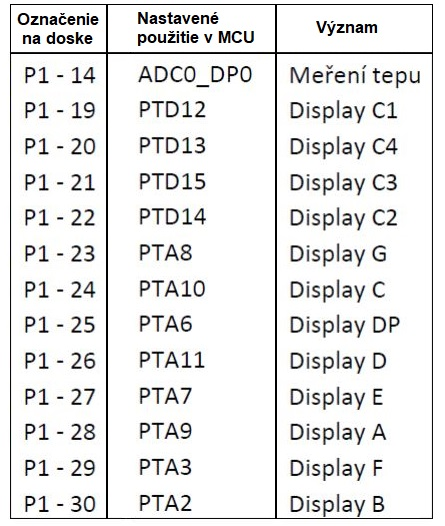
\includegraphics[scale=0.80]{piny.jpg}}
		\caption{Význam zapojenia}
		\label{pins}
	\end{figure}	
	\newpage
	\section{Implementácia}
	Implementácia sa nachádza v súbore \emph{main.c}. Na vytvorenie projektu bolo použité IDE Kinetis Design Studio.
	
	\subsection{Použité komponenty}
	\subsubsection{GPIO}
	\emph{General-purpose input/output}  slúži na nastavenie vstupných a výstupných pinov a následný zápis na piny LED displeja.
	\subsubsection{ADC}
	\emph{Analog-to-digital converter} je systém, ktorý v tomto projekte slúži na čítanie analógového signálu zo senzoru a jeho následný prevod do digitálnej podoby.
	\subsubsection{LPTMR}
	\emph{Low-Power Timer} je časovač, ktorý v tomto projekte slúži na vytvorenie prerušenia každých 15 sekúnd.
	\subsubsection{Clock}
	
	\subsection{Priebeh programu}
	Spočiatku sa inicializujú všetky používané piny, clocky, ADC prevodník a Low-Power časovač (LP0 clock, CMR - prerušenie každých 15 sekúnd). Vo while cykle sa čaká na ADC prevodník, kým neukončí konverziu dát, ktoré mu poslal senzor na kanáli DP0. Tieto dáta sa preženú cez high-pass filter, (aby sa vyrušil nízkofrekvenčný šum) a uložia do pola. Keď sa pole naplní, hodnoty v ňom sa spriemerujú pomocou metódy kĺzavého priemeru, pre jemnejšie vyhladenie signálu. Následne sa hodnota priradí ako aktuálna a porovná sa s predchádzajúcou hodnotou. Ak je aktuálna hodnota vyššia ako predchádzajúca, signál stúpa. V opačnom prípade signál klesá. V prípade, kedy stúpajúci signál začne klesať sa zaznamená jeden tlkot srdca. Aktuálna hodnota sa následne priradí do premennej, ktorá reprezentuje predchádzajúcu hodotu. Ak je čo vypísať, tak sa na konci cyklu while sa vypíše výsledok na displej pomocou funkcií \emph{show() (výber číslice)} a \emph{display\_val() (výber čísla)}. Po uplynutí 15-tich sekúnd nastane prerušenie vytvorené Low-Power časovačom, v ktorom sa zapíše výsledný počet tlkotov srdca do premennej \emph{result}, ktorá je vypisovaná na displej a časovač sa resetuje na vytvorenie ďalšieho prerušenia po 15-tich sekundách.
	
	\newpage
	\section{Záver}
	Projekt obsahuje implementáciu riešenia podľa požiadavok v zadaní. Pre presné meranie je dôležité, aby sa s prstom a senzorom nehýbalo.
	Pri testovaní bola funkčnosť overená porovnaním výsledku z displeja s tlakomerom~\ref{comparasion}.
	
	\begin{figure}[h] 
		\centering
		\subfigure{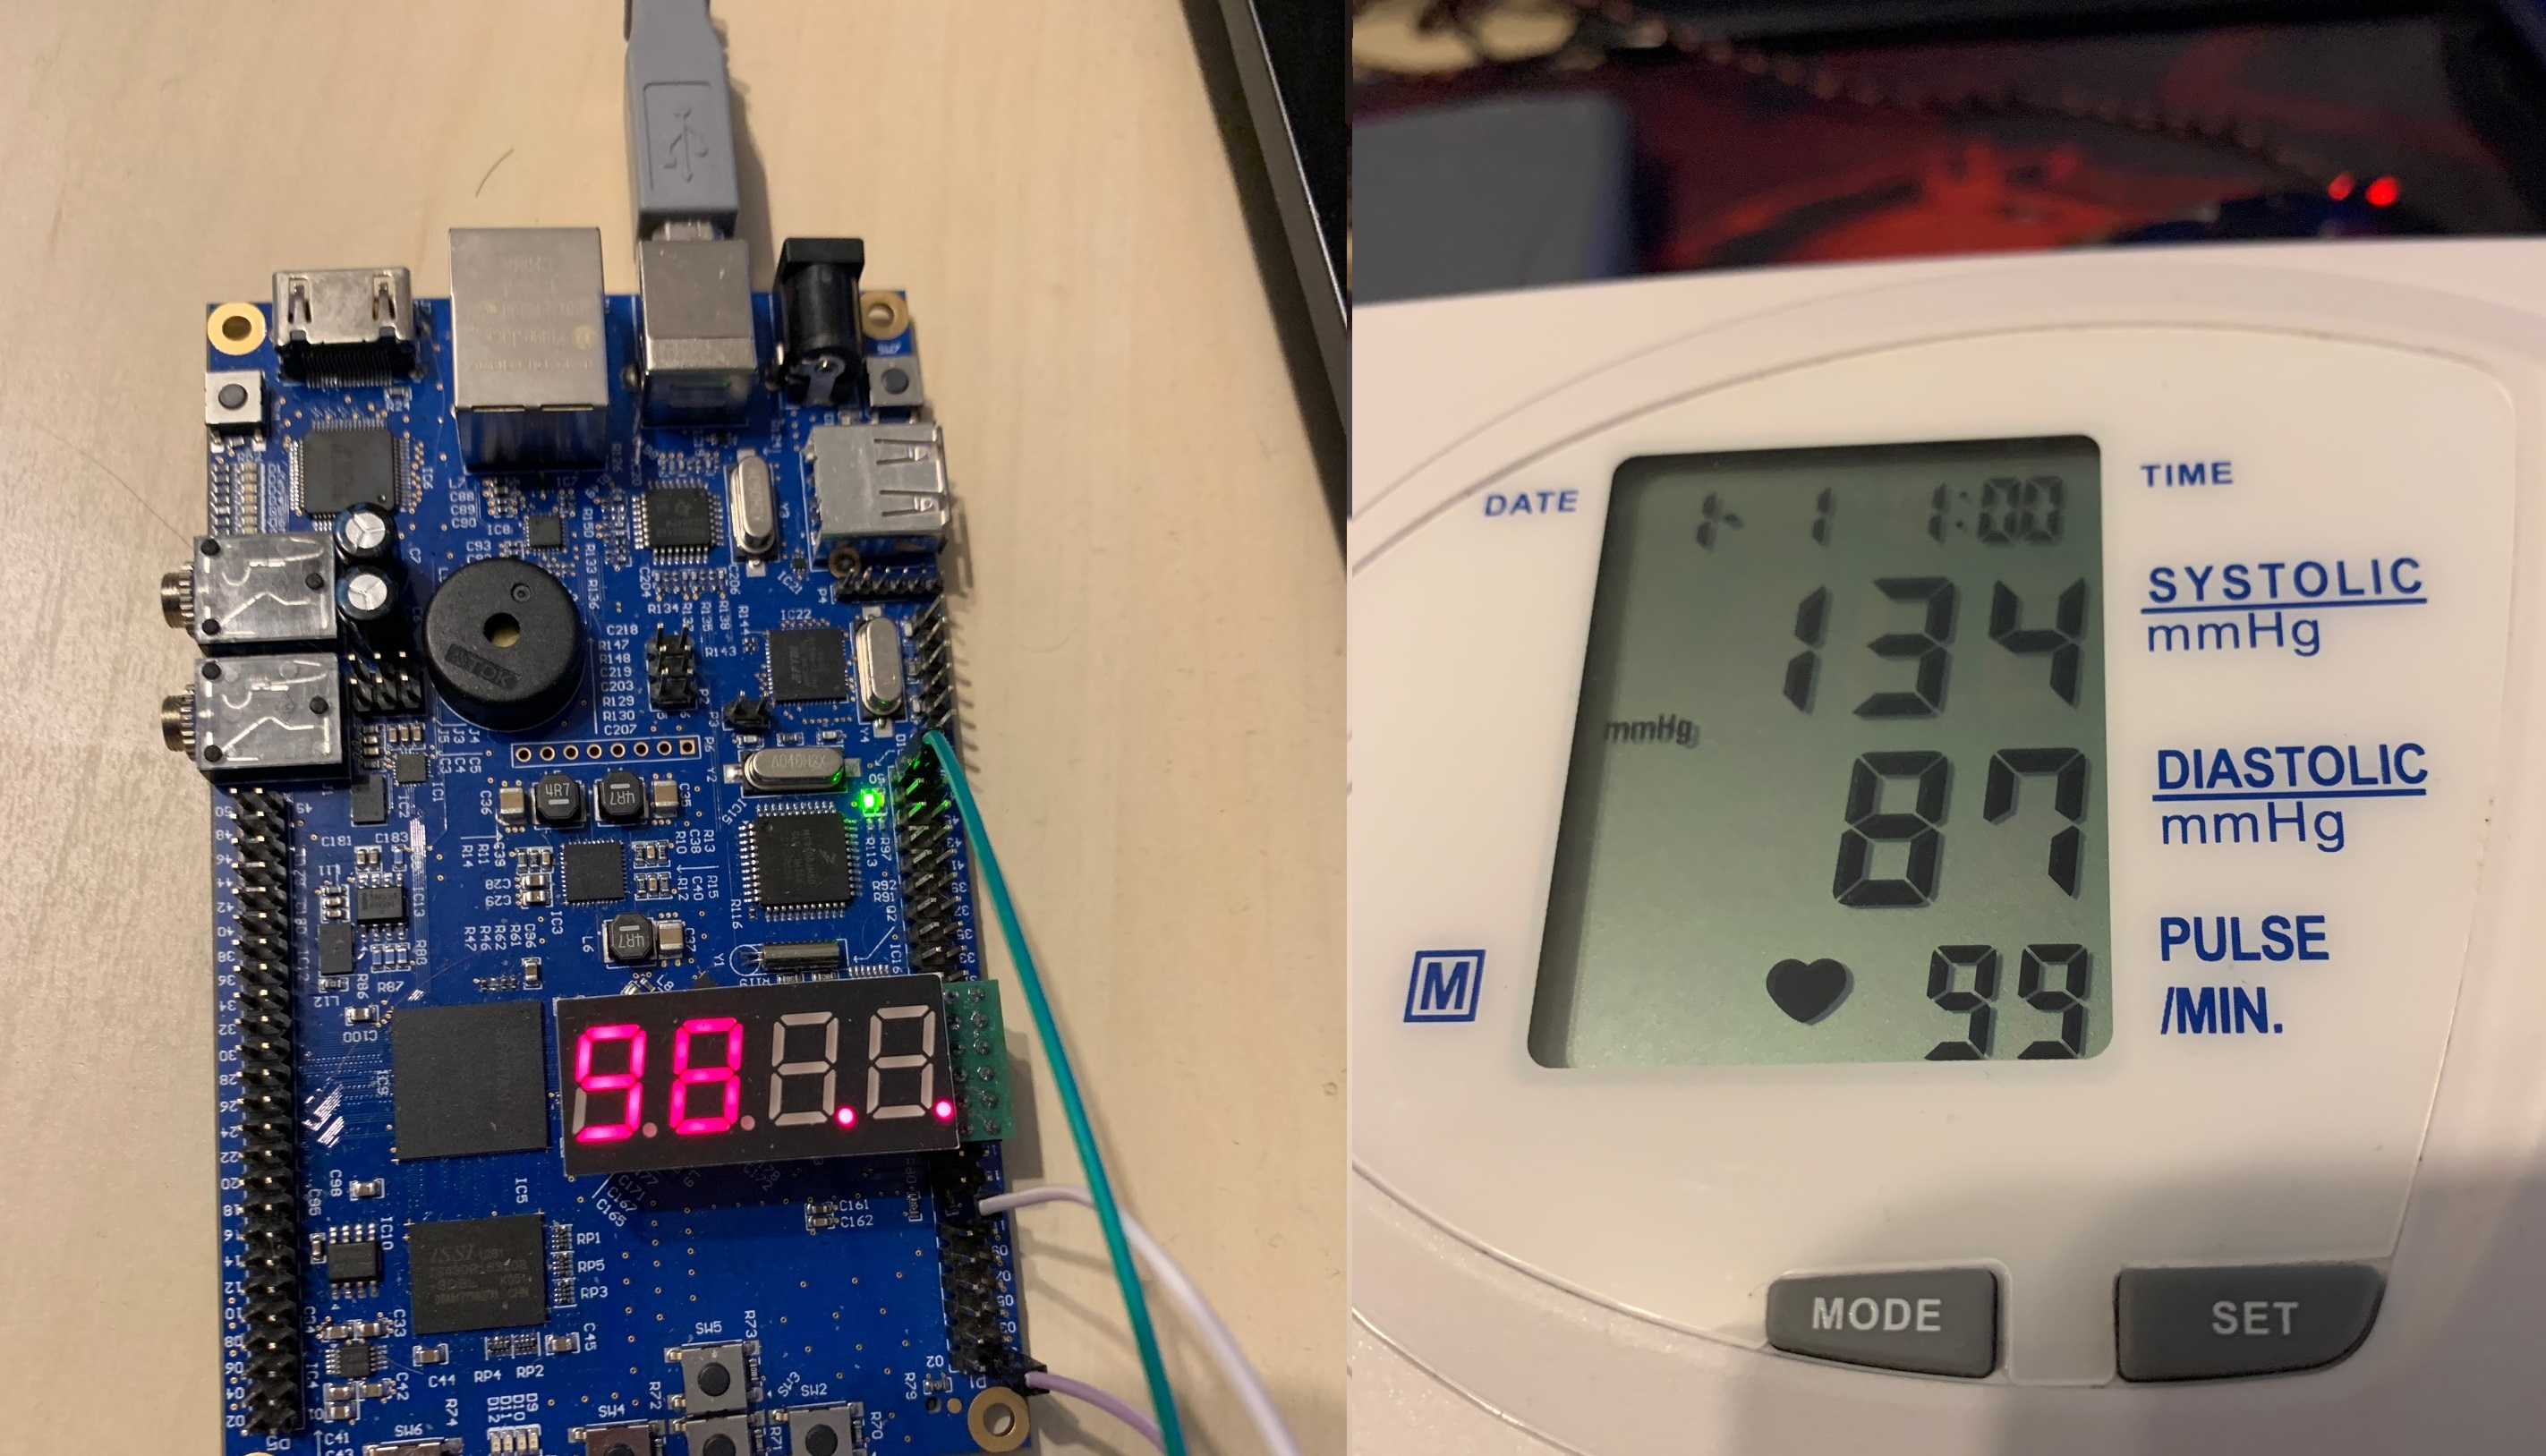
\includegraphics[scale=0.15]{comparasion.jpg}}
		\caption{Porovnanie výsledku z displeja s tlakomerom}
		\label{comparasion}
	\end{figure}	
	
	Autoevaluáciu projektu hodnotím na E-1, F-5, Q-3, P-1, D-4.
	
	\section{Odkaz k prezentácií}
	\href{https://nextcloud.fit.vutbr.cz/s/N6Rdnic3a63nriG}{Link na video: https://nextcloud.fit.vutbr.cz/s/N6Rdnic3a63nriG}

	\nocite{*}
    	\bibliographystyle{czechiso}
    	\renewcommand{\refname}{Literatúra}
    	\bibliography{biblib}
\end{document}
